\subsection{Regular Expressions in Streaming}
\begin{frame}
  \centering
  {\Large Streaming Regular Expression Membership and Pattern Matching}

  \bigskip
  {\large SODA'22}\\
  \bigskip
  
\includegraphics{pictures/mindmap/regexp.png}

  \bigskip
  Bartłomiej Dudek, Paweł Gawrychowski, Tatiana Starikovskaya
\end{frame}


\begin{frame}{}

    \begin{myalertblock}{Dudek, Gawrychowski, Gourdel, Starikovskaya, SODA'22}
        For any regular expression $R$ with $d$ occurrences of $|$ and $\ast$, we can solve regular expression membership on a text of length $n$ using $\Oh(d^{3}\polylog n)$ space and $\Oh(nd^{5}\polylog n)$ time per character.
    \end{myalertblock}
    
    \medskip
    \btheme{Main steps:}
    
    \begin{itemize}
    \item Define atomic strings: ``words" in the regular expression.
    
    \item Store efficiently specific occurrences of prefixes of atomic strings.
    
    \item Link those occurences stored to test if there is a ``partial" match of $R$.
    
    \item Translate this in a graph problem.
    
    \item Solve this problem efficiently by a circuit machinery!
    \end{itemize} 
    We also improve the circuit framework.
\end{frame}


\begin{frame}{Streaming pattern matching}
    \begin{mylemblock}{Porat and Porat, FOCS'09}
    $\Oh(\log m\cdot \log n)$ bits of space, $\Oh(\log m)$ time per position.
    \end{mylemblock}


    \bigskip
    \bblue{Main idea:} Given an algorithm $\mathcal{A}_{k}$ which generates all occurrences of
    $P[1..2^{k}]$, we will develop a new algorithm
    $\mathcal{A}_{k+1}$ which generates all occurrences of $P[1..2^{k+1}]$ using just $\Oh(\log n)$ bits of additional memory.
    
    \medskip
    \begin{overlayarea}{\textwidth}{3.5cm}
    \begin{center}
    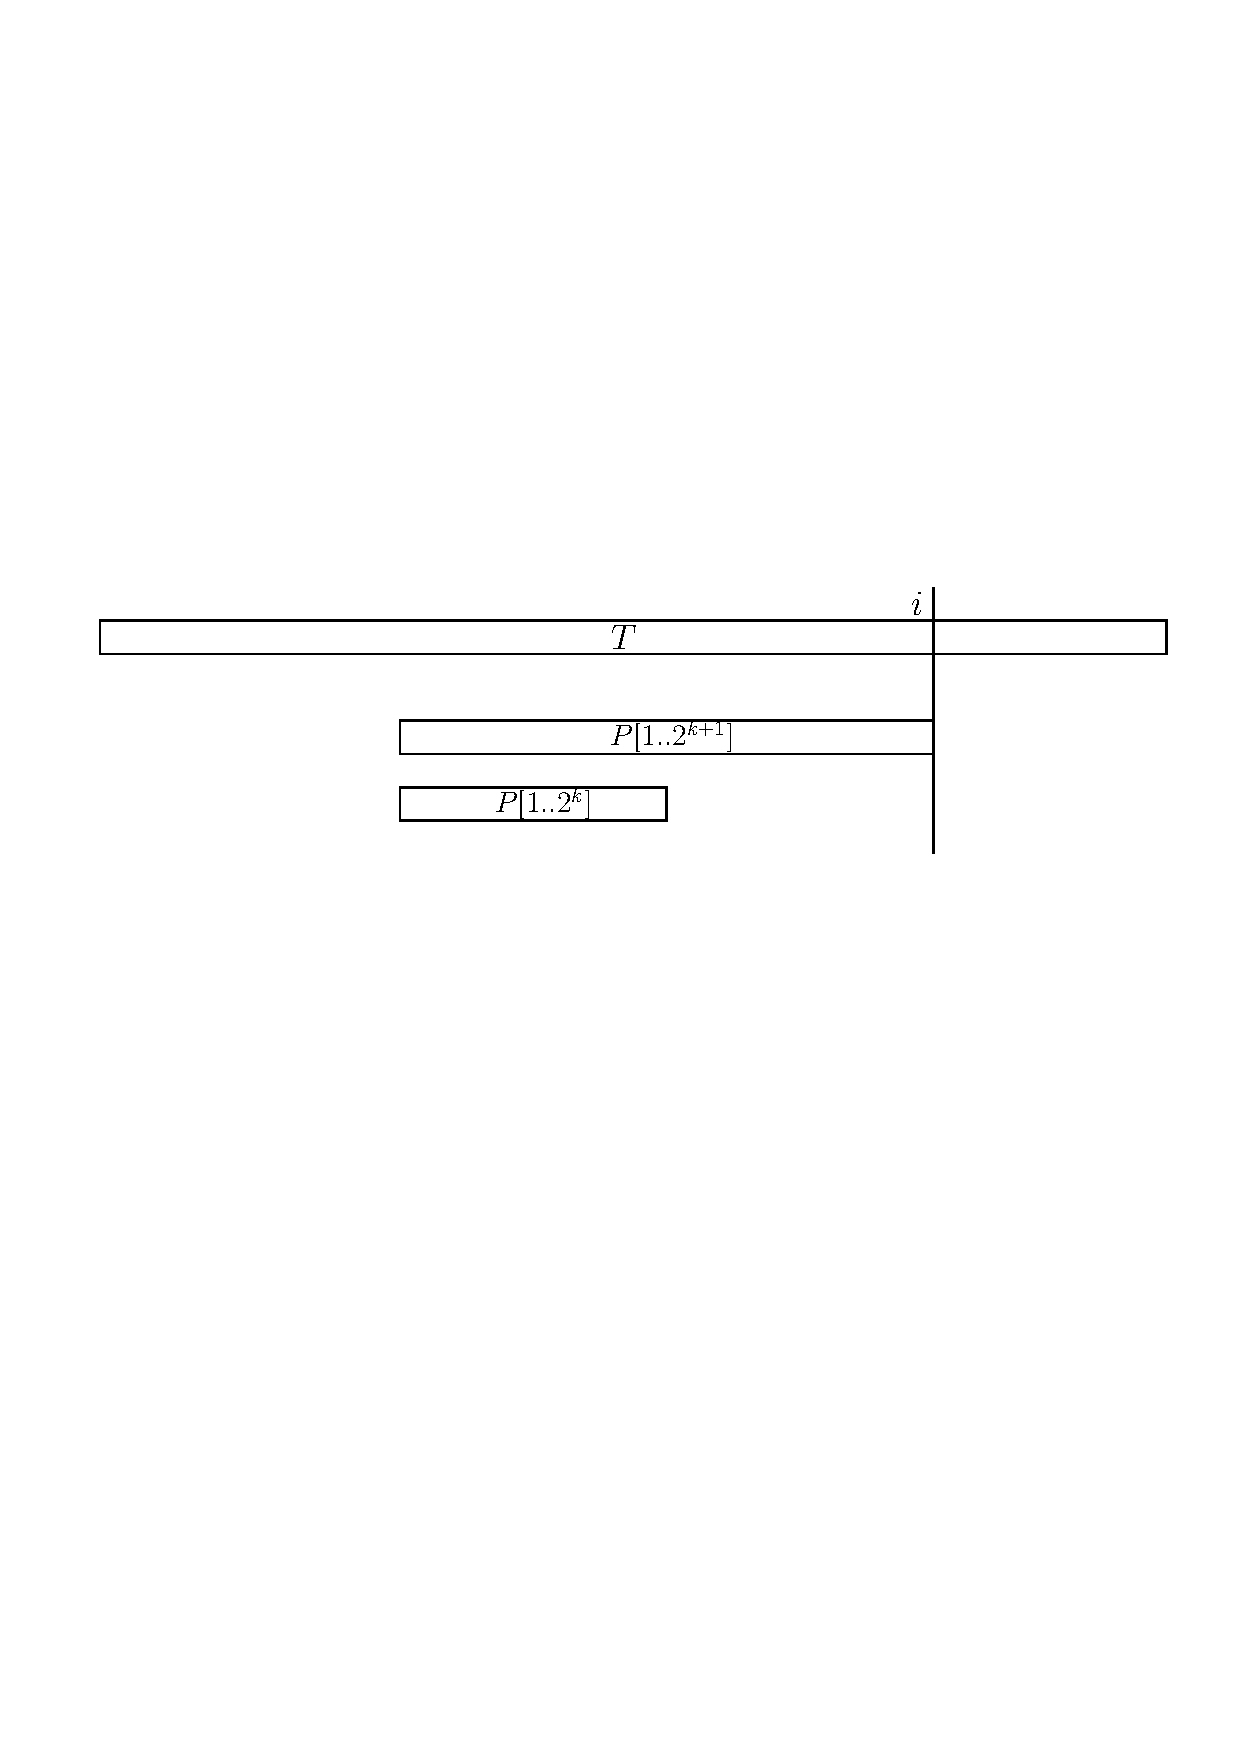
\includegraphics[width=0.7\textwidth]{pictures/more}
    \end{center}
    \end{overlayarea}
    \centering \textcolor{red}{\textbf{But...}\beamermathcolor{red} What if we have may occurrences of $P[1..2^{k}]$ in the window of size $2^{k+1}$?}
    \end{frame}
    
    
    %%%%%%%%%%%%%%%%%%%%%%%%%%%%%%%%%%%%%%%%%%%%%%%%%%%%%%%%%
    
    \begin{frame}
    
    {\beamermathcolor{red} What if we have may occurrences of $P[1..2^{k}]$ in the window of size $2^{k+1}$?}
    
    \begin{center}
    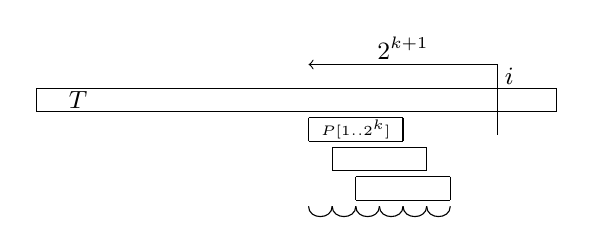
\begin{tikzpicture}[scale=0.3]
            \node  (0) at (-13.5, 1) {};
            \node  (1) at (-13.5, 0) {};
            \node  (2) at (8.5, 0) {};
            \node  (3) at (8.5, 1) {};
            \node  (4) at (-13.5, 1) {};
            \node  (5) at (8.5, 1) {};
            \node  (6) at (-13.5, 1) {};
            \node  (7) at (8.5, 1) {};
            \node  (8) at (8.5, 1) {};
            \node  (9) at (6, 2) {};
            \node  (10) at (6, -1) {};
            \node  (11) at (5.5, 1.5) {};
            \node  (12) at (6.5, 1.5) {\small{$i$}};
            \node  (13) at (5.5, 1.5) {};
            \node  (16) at (-11.75, 0.5) {\small{$T$}};
            \node  (17) at (-2, 2) {};
            \node  (18) at (-2, 2) {};
            \node  (19) at (2, 2.5) {};
            \node  (20) at (2, 2.7) {\small{$2^{k+1}$}};
            \node  (21) at (-2, -0.25) {};
            \node  (22) at (2, -0.25) {};
            \node  (23) at (2, -1.25) {};
            \node  (24) at (-2, -1.25) {};
            \node  (26) at (0, -0.75) {\tiny{$P[1..2^k]$}};
            \node  (27) at (-1, -1.5) {};
            \node  (28) at (3, -1.5) {};
            \node  (29) at (3, -2.5) {};
            \node  (30) at (-1, -2.5) {};
            \node  (33) at (0, -2.75) {};
            \node  (34) at (4, -2.75) {};
            \node  (35) at (4, -3.75) {};
            \node  (36) at (0, -3.75) {};
            \node  (37) at (-2, -4) {};
            \node  (38) at (-1, -4) {};
            \node  (39) at (0, -4) {};
            \node  (40) at (1, -4) {};
            \node  (41) at (2, -4) {};
            \node  (42) at (3, -4) {};
            \node  (43) at (4, -4) {};
            \node  (44) at (-1, -4) {};
            \node  (45) at (0, -4) {};
            \node  (46) at (0, -4) {};
            \node  (47) at (1, -4) {};
            \node  (48) at (2, -4) {};
            \node  (49) at (1, -4) {};
            \node  (50) at (2, -4) {};
            \node  (51) at (2, -4) {};
            \node  (52) at (3, -4) {};
            \node  (53) at (4, -4) {};
            \node  (54) at (3, -4) {};
            \node  (55) at (4, -4) {};
            \draw (6.center) to (8.center);
            \draw (6.center) to (1.center);
            \draw (1.center) to (2.center);
            \draw (8.center) to (2.center);
            \draw [in=90, out=-90] (9.center) to (10.center);
            \draw (21.center) to (22.center);
            \draw (22.center) to (23.center);
            \draw (21.center) to (24.center);
            \draw (24.center) to (23.center);
            \draw (27.center) to (28.center);
            \draw (28.center) to (29.center);
            \draw (27.center) to (30.center);
            \draw (30.center) to (29.center);
            \draw[<-] (18.center) to (9.center);
            \draw (33.center) to (34.center);
            \draw (34.center) to (35.center);
            \draw (33.center) to (36.center);
            \draw (36.center) to (35.center);
            
            \draw [bend right=90, looseness=1.50] (37.center) to (38.center);
            \draw [bend right=90, looseness=1.50] (44.center) to (45.center);
            \draw [bend right=90, looseness=1.50] (46.center) to (47.center);
            \draw [bend right=90, looseness=1.50] (49.center) to (50.center);
            \draw [bend right=90, looseness=1.50] (51.center) to (52.center);
            \draw [bend right=90, looseness=1.50] (54.center) to (55.center);
    \end{tikzpicture}
    \end{center}
    
    
    \textcolor{red}{Then there is periodicity!}  
    The occurences can be stored efficiently:
    \begin{itemize}
    
    \item The start, the period, and the number of repetitions
    
    \item The fingerprint of the prefix of the text up to the start of the progression and the fingerprint of the period
    \end{itemize}
    
    \medskip
    
    
    {
        \beamermathcolor{red}
        \alert{$\Oh(\log n)$ bits of space per level!}  \\ 
        \footnotesize{Correctness: if $P$ occurs, all $\log m$ prefixes will be there too and be detected w.h.p.}
    }

\end{frame}


\begin{frame}

\begin{exampleblock}{Main idea}
We run a separate pattern matching process for each of the atomic strings, and store some of the found occurrences as witnesses.
\end{exampleblock}

\pause
\begin{block}{Witness}
Let $P$ be a prefix of length $2^{i}$ of some atomic string that occurs ending at position $r$ in $T$. Then, $r$ is a witness
if $T[1..r]$ is a partial occurrence of $R$ ending at $P$.
\end{block}
\pause

This works \ntheme{if everything is aperiodic:}\pause \\
there are only a constant number of witnesses for each prefix.\\
\pause

\vfill
\textcolor{red}{However, this is not always the case...}

\end{frame}
    
    
    
%%%%%%%%%%%%%%%%%%%%%%%%%%%%%%%%%%%%%%%%%%%%%%%%%%%%%%%%% 
% General witness


\begin{frame} 
\ntheme{For the general case:}
\begin{itemize}
\pause
\item Periodic atomic string will be found in periodic regions of the text.
\pause
\item We keep some occurrences of earlier atomic strings on an accepting path (check acceptance via a graph problem).
\pause 
\item We carefully chose them to always be able to bound their number.
\end{itemize}
\pause

\begin{center}
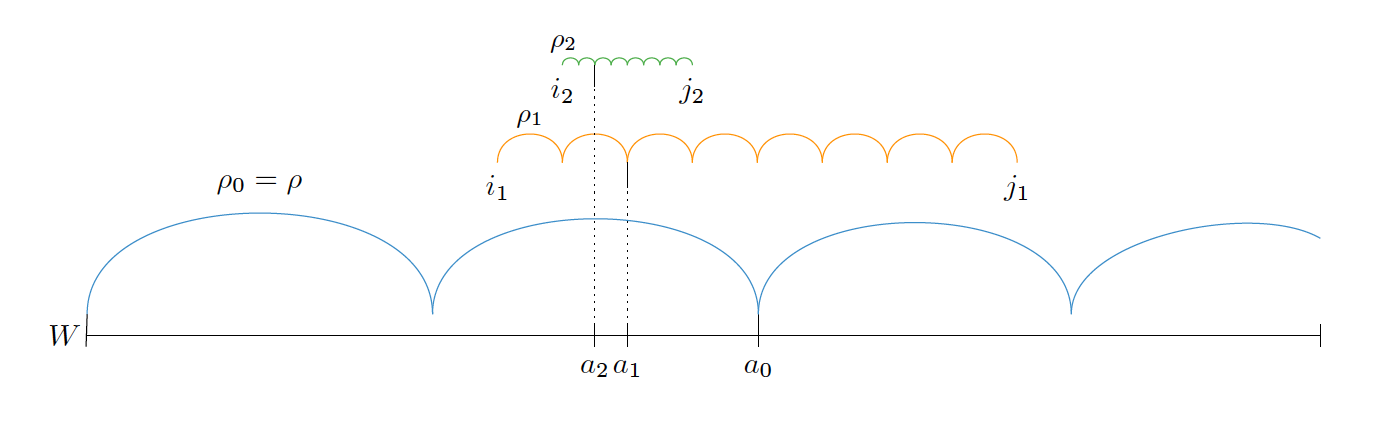
\includegraphics[width=\textwidth]{pictures/anchors.png}
\end{center}
\pause

\ntheme{Main novelty:} Treat the non-periodic and periodic cases together with a reasoning $\Oh(\log n)$ levels.

\end{frame}

\begin{frame}{Circuit framework}
    $$C_k[u,v][d]=\bigvee_{\substack{w\in V(G) \\  i\in \{0,\ldots,d\}}} C_{k-1}[u,w][i] \wedge C_{k-1}[w,v][d-i]$$
    
     
     
    \begin{block}{Lokshtanov and Nederlof, STOC'10; Bringmann, SODA'17}
    Consider a circuit $C$ with every gate being an addition or convolution gate and computing a vectors of the same length.
    Assuming that no convolution gate overflows,
    we can efficiently compute an entry of the output vector in space depending on the size of the circuit
    (and not the length of the vectors).
    \end{block}
    
    
    \begin{alertblock}{}
    We remove the dependency on the Extended Riemann Hypothesis, replacing it with an application of the Bombieri--Vinogradov theorem.\\ 
    %
    %(a major result of analytic number theory, obtained in the mid-1960s, concerning the distribution of primes in arithmetic progressions)
    \end{alertblock}
    
\end{frame}
    